\documentclass[sigconf]{acmart}

\usepackage[english]{babel}
\usepackage{blindtext}

% Copyright
\renewcommand\footnotetextcopyrightpermission[1]{} % removes footnote with conference info
\setcopyright{none}
%\setcopyright{acmcopyright}
%\setcopyright{acmlicensed}
%\setcopyright{rightsretained}
%\setcopyright{usgov}
%\setcopyright{usgovmixed}
%\setcopyright{cagov}
%\setcopyright{cagovmixed}

\settopmatter{printacmref=false, printccs=false, printfolios=false}

% DOI
\acmDOI{}

% ISBN
\acmISBN{}

%Conference
%\acmConference[Submitted for review to SIGCOMM]{}
%\acmYear{2018}
%\copyrightyear{}

%% {} with no args suppresses printing of the price
\acmPrice{}


\begin{document}
\title{Reproduction: Measuring the Security Harm of TLS Crypto Shortcuts}

%\titlenote{Produces the permission block, and copyright information}
%\subtitle{Extended Abstract}

\author{Jared Crawford}
% \authornote{Note}
% \orcid{1234-5678-9012}
\affiliation{%
  \institution{Stanford University}
  \streetaddress{450 Serra Mall}
  \city{Stanford} 
  \state{California} 
  \postcode{94305}
}
\email{jared13@stanford.edu}

% The default list of authors is too long for headers}
\renewcommand{\shortauthors}{Crawford}

\begin{abstract}
    Server authenticity, privacy over communication lines, and integrity of transport level data are desirable for many popular applications such as web browsing, email, and Voice over IP. 
    The Transport Layer Security protocol (TLS) provides these security properties between application servers and web browsers through various cryptographic primitives. 
    A typical connection over TLSv1.2 today is a multistep interactive process between server and client which includes an exchange of public key information, a negotiation on which ciphers to use for the resulting communication, and advertisement for support of a variety of TLS extensions. 
    Thus, establishing this secure communication line incurs an initial latency overhead in the form of multiple transport level handshake round trip times. 
    
    
    \begin{figure}[hp]
    \centering
    \includegraphics[width=\linewidth]{figures/handshake.png}
    \caption{A diagram from Tobarra et. al. demonstrating the latency overhead incurred by TLS handshakes \cite{handshake}. An insecure alternative such as TCP needs only a three way handshake which will typically complete more quickly than a TLS handshake.}
    \end{figure}
    
    As a performance optimization for the common case of bursty connections in frequent but short intervals, TLS supports extensions which allow a web browser to resume a previous connection with a server without completing a new handshake. However, these mechanisms trade off with an important security property of user traffic: perfect forward secrecy. In a perfect forward secret scheme, each separate server-client connection is encrypted using a unique session key. Immediately after the connection terminates, both parties are responsible for deleting the key. Once the ephemeral key has been deleted, the contents of this communication cannot be decrypted even in the event of server compromise. However, in an imperfect secret scheme, one party will maintain a temporary cache of session state including the session key to allow frequent reconnections to complete more quickly. By maintaining session state across connections, a client can resume subsequent connections without having to renegotiate ciphers and derive a new session key. The maximum lifetime of a session key is thus a tradeoff between privacy and reconnect latency in such a scheme.
    
   
\end{abstract}

\maketitle

\section{Introduction}

The authors made TLS 1.2 handshakes over a nine week period with the Alexa Top Million sites and studied the reuse of private ephemeral values in TLS session resumption, TLS session tickets, and Diffie Helmann key exchange. In addition, the researchers observed more general trends such as the churn of the top million sites and protocol usage statistics. In this report, I present a reproduction of these results two years after the papers publication. Due to time constraints, the data collected spans a comparatively smaller one week period compared to the original paper.

The key results of this paper which I reproduce are Figures 1-4 in the paper. TLS supports user advertised lifetimes of ephemeral secrets. For example, a client can specify that their session key should be deleted after 1 hour to maintain a higher degree of forward secrecy. Figures 1-2 demonstrate how compliants sites are with these advertised ephemeral lifetimes. Figures 3-4 show how long (in days) that session ticket encryption keys are reused by sites. Reuse of encryption keys expose users to additional risk because it requires that the server save a copy of these keys for their lifetime. Thus, if a malicious party gains server-side access to a site which reuses keys for one week, client communications during the past week can be retroactively decrypted. Additionally, I present a summary of what TLS features are supported by popular domains (e.g. "of the Majestic Million websites that support HTTPS, 83\% support session ID resumption and 76\% support session tickets.") This data for this analyisis was collected over a one week day period from May 26 to June 2.

Churn Figure
\begin{figure}[tp]
\centering
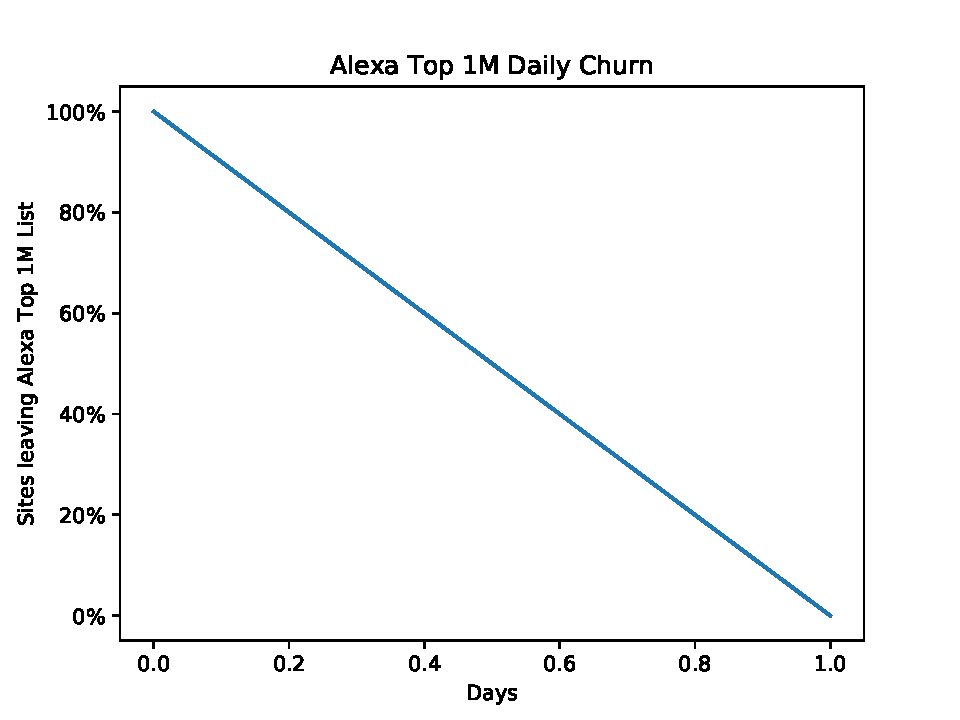
\includegraphics{figures/churn.png}
\caption{\blindtext}
\end{figure}


\section{Reproductions}

\subsection{Figures 1-2}
Figure 1
\begin{figure}[tp]
\centering
\includegraphics{figures/id_minutely_cdf.png}
\caption{\blindtext}
\end{figure}

Figure 2
\begin{figure}[tp]
\centering
\includegraphics{figures/stek_minutely_cdf.png}
\caption{\blindtext}
\end{figure}

\subsection{Figures 3-4}
Figure 3
\begin{figure}[tp]
\centering
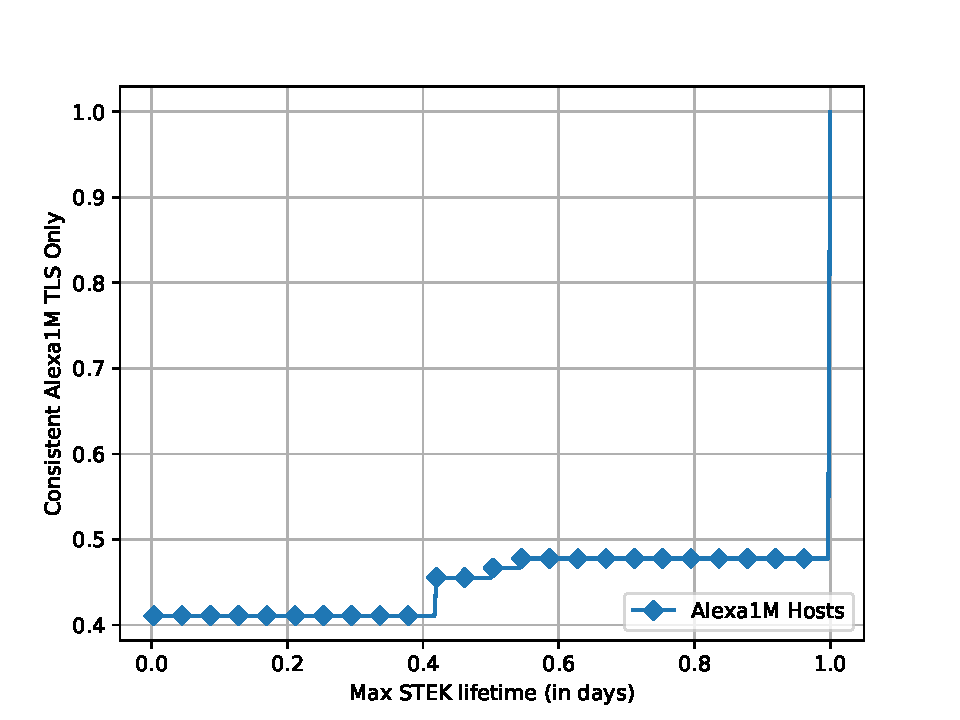
\includegraphics{figures/max_stek_cdf.png}
\caption{\blindtext}
\end{figure}

Figure 4
\begin{figure}[tp]
\centering
\includegraphics{figures/stek_stacked.png}
\caption{\blindtext}
\end{figure}

\section{Evaluation}

\section{Conclusion}

\bibliographystyle{ACM-Reference-Format}
\bibliography{reference}

\end{document}